%
%
%
\chapter{Modelagem Matemática} \label{chap:moddesenvolvidos}


\emph{Modelos matemáticos de colunas de destilação podem ser classificados de acordo com o seu grau de detalhamento:
se possuem predição da composição, temperatura e vazões para cada prato, são chamados de modelos rigorosos. Se são
compostos por uma descrição global da coluna utilizando um menor número de variáveis, baseados em algum tipo de
interpolação, são ditos modelos reduzidos \cite{Fletcher:2000}. Neste trabalho, os modelos desenvolvidos fazem parte do
primeiro
grupo, modelos rigorosos, prato-a-prato, baseados na consideração de equilíbrio termodinâmico entre as fases líquida e
vapor.
}

\section{Introdução}

Para o desenvolvimento de um modelo de coluna de destilação, diversos modelos
de equipamentos periféricos são necessários. Exemplos destes equipamentos são:
bomba, válvula, tanques, condensador e referverdor.
Neste capítulo, os modelos desenvolvidos são apresentados, com suas
considerações e equacionamento.

Além dos modelos dos equipamentos individuais, é apresentado um estudo a
respeito de correlações hidráulicas disponíveis na literatura para o cálculo
das vazões internas da coluna.

Para a implementação dos modelos e simulações foi utilizado o software \emso\
(\emsoname) que é uma ferramenta de modelagem, simulação e
otimização de processos.
O simulador \emso\ pode ser utilizado de forma genérica e nos mais variados
ramos da engenharia. Apresenta várias características importantes que auxiliam
no desenvolvimento de modelos e na realização de simulações como: análise de
consistência de unidades de medida, verificação de singularidades do sistema e
consistência das condições iniciais. Mais detalhes sobre o simulador são
apresentados no \autoref{ap:emso} desta dissertação.

% Um sistema de separação, como por exemplo uma coluna de destilação, é formado por um conjunto de equipamentos. Para cada
% um dos equipamentos mais comuns encontrados nesse tipo de sistema foram confeccionados modelos que tentam prever o
% comportamento dinâmico e$\setminus$ou estacionário dos mesmos. Estes modelos serão apresentados a seguir nas próximas
% seções.

% \section{Bomba e Divisor de correntes}

\section{Bomba} \label{sec:modelobomba}
Neste trabalho um modelo simplificado de bomba foi construído.
Este modelo é utilizado apenas para reintroduzir na coluna de destilação a corrente de destilado em uma pressão maior
que a do prato do topo. Desta forma, este modelo inclui apenas um acréscimo de pressão da sua corrente de saída com
relação à corrente de entrada.
Sua representação esquemática pode ser vista na \autoref{fig:esquemapump}:

\begin{figure}[htb]
\centering 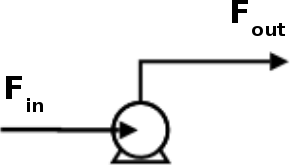
\includegraphics[scale=0.5]{images/Chap3/esquemapump2.png}
\caption{Modelo esquemático de uma bomba}
\label{fig:esquemapump}
\end{figure}

Trata-se de um modelo simplificado, onde o usuário fornece uma queda de pressão $\Delta P$ e é composto pelas equações:

\begin{flushleft}
Balanço de massa:
\end{flushleft}
\begin{equation}
F_{in} = F_{out}
\end{equation}
\begin{equation}
z_{in_i} = z_{out_i}  \qquad i=1,2,\cdots,c
\end{equation}
\nomenclature{$F_{in}$}{Vazão molar que entra no equipamento \nomunit{mol/s}}
\nomenclature{$F_{out}$}{Vazão molar que sai do equipamento \nomunit{mol/s}}
\nomenclature{$z_{in}$}{Vetor de frações molares dos componentes da corrente que entra no equipamento}
\nomenclature{$z_{out}$}{Vetor de frações molares dos componentes da corrente que sai do equipamento}
\nomenclature{$z_{in_i}$}{Fração molar do componente $i$ na corrente que entra no equipamento}
\nomenclature{$z_{out_i}$}{Fração molar do componente $i$ na corrente que sai do equipamento}
Pressão:
\begin{equation}
P_{out} = P_{in} + \Delta P
\end{equation}
\nomenclature{$P_{out}$}{Pressão da corrente que sai do equipamento \nomunit{atm}}
\nomenclature{$P_{in}$}{Pressão da corrente que entra do equipamento \nomunit{atm}}
% \nomenclature{$dP$}{Queda de pressão no equipamento ($atm$)}
Entalpia:
\begin{equation}
h_{out} = h_{in} + \dfrac{\Delta P}{\rho} \cdot Mw
\end{equation}
Massa Específica:
\begin{equation}
\dfrac{1}{\rho} = \dfrac{(1-v)}{\rho^L} + \dfrac{v}{\rho^V}
\end{equation}
% onde as composições das fases líquida e vapor na saída da bomba, necessárias para o cálculo da fração
% vaporizada e das propriedades físicas são obtidas através da solução de um \textit{flash PH}.
onde $Mw$ é a massa molar média da mistura, $v$ é a fração vaporizada da corrente, $\rho$ é a massa específica e
os superscritos $L$ e $V$ são utilizados para especificar o caso líquido e
vapor, respectivamente.

Adicionalmente às equações acima, a temperatura e a fração
vaporizada da corrente que sai da bomba são calculadas pelo pacote
termodinâmico através de um cálculo de \textit{flash}.
Isto é necessário para
que todas as informações da corrente de saída da bomba estejam disponíveis, permitindo que esta seja conectada
a qualquer outro modelo desenvolvido no EMSO.
Isto poderá ser visualizado mais adiante, quando for construído o modelo de uma
coluna de destilação completa.

\nomenclature{$T_{out}$}{Temperatura da corrente que sai do equipamento \nomunit{K}}
\nomenclature{$T_{in}$}{Temperatura da corrente que entra do equipamento \nomunit{K}}
\nomenclature[G]{$\rho$}{Massa específica da corrente \nomunit{kg/m^3}}

Na linguagem do simulador \emso\ o modelo acima apresentado pode ser escrito
conforme o \autoref{code:bomba}: \lstinputlisting[firstline=3, lastline=33, numbers=none, language=EMSO, caption=Modelo simplificado de bomba. , label=code:bomba] {images/Chap4/pump.mso}

Deve-se ficar atento ao fato de que, em algumas equações, se faz uso de funções externas ao simulador, no caso
funções de \textit{plugins}. No \autoref{code:bomba}, isto acontece no cálculo da massa específica, onde a
densidade da mistura na fase líquida e na fase vapor são calculadas através de funções do \textit{plugin} PP
que foi previamente declarado na seção de parâmetros. Este \textit{plugin} consiste é um pacote termodinâmico
que realiza os cálculos de propriedades físicas e termodinâmicas da mistura a ser simulada. Praticamente todos os
modelos apresentados aqui necessitam de alguma cálculo deste tipo.


\section{Divisor de correntes: \textit{splitter}} \label{sec:modelosplitter}
\textit{Splitter} é um divisor de correntes, utilizado em modelos de colunas de destilação para separar a corrente
de topo em destilado e refluxo e para separar o produto de fundo da corrente que volta para
o refervedor.

Um \textit{splitter} pode ser representado pela \autoref{fig:splitter}, onde a corrente de entrada se
separa em duas correntes de saída. Um parâmetro fixado pelo usuário, chamado $frac$, determina qual proporção da vazão de
entrada vai para a corrente $out1$.
\begin{figure}[htb]
\centering 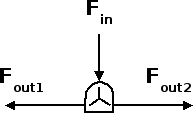
\includegraphics[scale=0.9]{images/Chap3/esquemasplitter2.png}
\caption{Modelo esquemático de um \textit{splitter}}
\label{fig:splitter}
\end{figure}

O modelo do \textit{splitter} é composto pelas seguintes equações:

\begin{flushleft}
Vazão:
\end{flushleft}
\begin{equation}
F_{out1} = F_{in} \cdot frac
\end{equation}
\begin{equation}
F_{out2} + F_{out1} = F_{in}
\end{equation}
\nomenclature{$frac$}{Fração de \textit{split} da vazão}
Temperatura:
\begin{equation}
T_{out1} = T_{in}
\end{equation}
\begin{equation}
T_{out2} = T_{in}
\end{equation}
Pressão:
\begin{equation}
P_{out1} = P_{in}
\end{equation}
\begin{equation}
P_{out2} = P_{in}
\end{equation}
Composição:
\begin{equation}
z_{out1_i} = z_{in_i} \qquad i=1,2,\cdots,c
\end{equation}
\begin{equation}
z_{out2_i} = z_{in_i} \qquad i=1,2,\cdots,c
\end{equation}
Entalpia:
\begin{equation}
h_{out1} = h_{in} \quad\textrm{ou}\quad h_{out1} = h(T_{out1}, P_{out1},
z_{out1})
\end{equation}
\begin{equation}
h_{out2} = h_{in} \quad\textrm{ou}\quad h_{out2} = h(T_{out2}, P_{out2},
z_{out2})
\end{equation}
Fração Vaporizada da corrente:
\begin{equation}
v_{out1} = v_{in} \quad\textrm{ou}\quad v_{out1} = v(T_{out1}, P_{out1},
z_{out1})
\end{equation}
\begin{equation}
v_{out2} = v_{in} \quad\textrm{ou}\quad v_{out2} = v(T_{out2}, P_{out2},
z_{out2})
\end{equation}
\nomenclature{$h_{out}$}{Entalpia da corrente que sai do equipamento \nomunit{J/mol}}
\nomenclature{$h_{in}$}{Entalpia da corrente que entra no equipamento \nomunit{J/mol}}

No \autoref{code:splitter}, pode-se ver a implementação do equacionamento acima
na linguagem do simulador \emso.
\lstinputlisting[firstline=68, lastline=96, numbers=none, language=EMSO, caption=Modelo de \textit{splitter}. ,
label=code:splitter] {images/Chap4/splitter.mso}

\section{Tanques de acúmulo}
Os tanques são responsáveis pelo acúmulo da maior parte da mistura que
se encontra no interior da coluna de destilação.
Neste trabalho, dois modelos foram desenvolvidos, apresentados a seguir.

\subsection{Tanque cilíndrico vertical} \label{sec:modelotanquecilindrico}
Neste trabalho o modelo dinâmico de um tanque cilíndrico vertical, como
representado na \autoref{fig:esquematank1}, foi construído.
Esse modelo considera apenas uma fase líquida misturada perfeitamente e que não
há perda de carga no bocal de alimentação.
Esse modelo é geralmente utilizado acoplado abaixo do prato de fundo da coluna, quando um refervedor termossifão é utilizado.

\begin{figure}[htb]
\centering 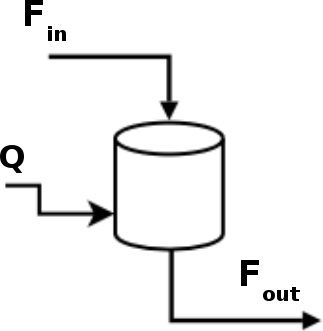
\includegraphics[scale=0.5]{images/Chap3/esquematank2.png}
\caption{Modelo esquemático de um tanque cilíndrico.}
\label{fig:esquematank1}
\end{figure}
O modelo é composto pelas seguintes equações:

\begin{flushleft}
Balanço molar por componente:
\end{flushleft}
\begin{equation}
\dfrac{dM_i}{dt} = F_{in} \cdot z_{in_i} - F_{out}  \cdot z_{out_i} \qquad i=1,2,\cdots,c
\end{equation}
% \nomenclature{$M$}{Acúmulo molar total ($mol$)}
\nomenclature{$M_i$}{Acúmulo molar do componente $i$ \nomunit{mol}}
\nomenclature{$M_k$}{Acúmulo molar do componente $k$ \nomunit{mol}}
Balanço de energia:
\begin{equation}
\dfrac{dE}{dt} = F_{in} \cdot h_{in} - F_{out}  \cdot h_{out} + Q
\end{equation}
\nomenclature{$E$}{Energia interna do sistema \nomunit{J}}
\nomenclature{$Q$}{Taxa de calor \nomunit{J/s}}
Acúmulo de energia:
\begin{equation}
E = \sum_i M_i \cdot h_{out}
\end{equation}
Relação entre acúmulos e composições:
\begin{equation}
M_i = z_{out_i} \cdot \sum_k M_k \qquad i=1,2,\cdots,c
\end{equation}
Sem perda de carga:
\begin{equation}
P_{out} = P_{in}
\end{equation}
Nível de líquido:
\begin{equation}
Level = \dfrac{\sum_i M_i \cdot v^L}{A_{cross}}
\end{equation}
\nomenclature{$v^L$}{Volume molar da fase líquida \nomunit{m^3/mol}}
\nomenclature{$v^V$}{Volume molar da fase vapor \nomunit{m^3/mol}}
\nomenclature{$v$}{Fração vaporizada da corrente}
\nomenclature{$Level$}{Nível de líquido \nomunit{m}}
\nomenclature{$A_{cross}$}{Área da seção transversal \nomunit{m^2}}

As propriedades físicas e termodinâmicas necessárias são calculadas através de rotinas externas,
baseadas no modelo termodinâmico adotado:
\begin{equation}
h_{out} = h(T_{out}, P_{out}, z_{out})
\end{equation}
\begin{equation}
v^L = v^L(T_{out}, P_{out}, z_{out})
\end{equation}

Na linguagem do simulador \emso\ o modelo acima apresentado assume a forma
mostrada no \autoref{code:tanquedepe}.
\lstinputlisting[firstline=10, lastline=49, numbers=none, language=EMSO, caption=Modelo de tanque de acúmulo. ,
label=code:tanquedepe] {images/Chap4/tank.mso}

\subsection{Tanque cilíndrico horizontal} \label{sec:modelotanquecilindrodeitado}
Este modelo se baseia nas mesmas considerações do modelo de tanque vertical,
porém apresenta a geometria de um cilindro deitado, como pode ser visto na \autoref{fig:esquematank2}:
\begin{figure}[htb]
\centering 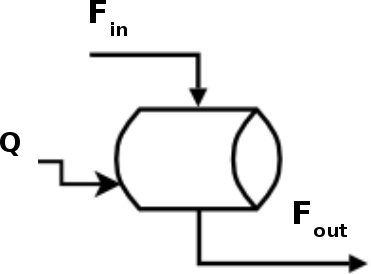
\includegraphics[scale=0.5]{images/Chap3/esquematank_22.png}
\caption{Modelo esquemático de um tanque cilíndrico deitado.}
\label{fig:esquematank2}
\end{figure}

No processo estudado no \autoref{chap:coldeiso}, este equipamento é utilizado no
topo da coluna, pois a dinâmica do condensador é muito rápida.
Nestes casos, este tanque serve como um pulmão para as bombas do refluxo e destilado.
Nos casos em que a dinâmica do condensador é muito rápida usualmente um modelo estacionário é utilizado,
como apresentado na \autoref{sec:modelocondensadorestacionario}.
Um modelo dinâmico de tanque cilíndrico horizontal pode ser composto pelas seguintes equações:

\begin{flushleft}
Balanço molar por componente:
\end{flushleft}
\begin{equation}
\dfrac{dM_i}{dt} = F_{in} \cdot z_{in_i} - F_{out}  \cdot z_{out_i}  \qquad i=1,2,\cdots,c
\end{equation}
Balanço de energia:
\begin{equation}
\dfrac{dE}{dt} = F_{in} \cdot h_{in} - F_{out}  \cdot h_{out} + Q
\end{equation}
Acúmulo de energia:
\begin{equation}
E = \sum_i M_i \cdot h_{out}
\end{equation}
Relação entre acúmulos e composições:
\begin{equation}
M_i = z_{out_i} \cdot \sum_j M_j \qquad i=1,2,\cdots,c
\end{equation}
Sem perda de carga:
\begin{equation}
P_{out} = P_{in}
\end{equation}
Área da seção transversal do cilindro deitado:
\begin{equation}
A_{cross} = r^2 \cdot \left( asin(1) - asin(\dfrac{r-Level}{r}) \right)  + (Level-r) \cdot \sqrt{Level \cdot (2 \cdot r - Level)}
\end{equation}
\nomenclature{$r$}{Raio \nomunit{m}}
\nomenclature{$L$}{Comprimento do tanque \nomunit{m}}
Acúmulo de líquido:
\begin{equation}
A_{cross} \cdot L = \sum_i M_i \cdot v^L
\end{equation}
As propriedades físicas e termodinâmicas necessárias são calculadas através de rotinas externas:
\begin{equation}
h_{out} = h(T_{out}, P_{out}, z_{out})
\end{equation}
\begin{equation}
v^L = v^L(T_{out}, P_{out}, z_{out})
\end{equation}
Este equacionamento, implementado no \emso, apresenta a seguinte estrutura
mostrada no \autoref{code:tanquedeitado}.
\lstinputlisting[firstline=50, lastline=95, numbers=none, language=EMSO, caption=Modelo de tanque cilíndrico deitado. ,
label=code:tanquedeitado] {images/Chap4/tank.mso}

\section{Refervedores}
Dois modelos de refervedor foram desenvolvidos: um modelo dinâmico, representando um refervedor do tipo
\textit{Kettle}; e um modelo estacionário correspondendo a um refervedor termossifão.

\subsection{Refervedor Dinâmico} \label{sec:modelorefervedordinamico}
O refervedor dinâmico aqui modelado pode ser representado pela \autoref{fig:esquemarebdin}. Como pode ser visto, o
refervedor recebe uma corrente de alimentação, no caso de destilações batelada, e uma corrente de líquido
proveniente da coluna. Possui como
saída duas correntes, uma líquida e outra vapor. Este refervedor é considerado como mais um estágio de
equilíbrio da coluna, em condição de mistura perfeita em ambas as fases.

\begin{figure}[htb]
\centering 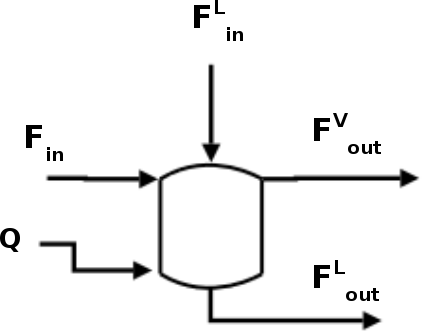
\includegraphics[scale=0.5]{images/Chap3/esquemareboiler2.png}
\caption{Modelo esquemático de um refervedor dinâmico.}
\label{fig:esquemarebdin}
\end{figure}

O modelo é composto pelas seguintes equações:

% \begin{flushleft}
Balanço molar por componente:
% \end{flushleft}
\begin{equation}
\dfrac{dM_i}{dt} = F_{in} \cdot z_{in_i} + F_{in}^L \cdot x_{in_i}- F_{out}^L  \cdot x_{out_i} - F_{out}^V \cdot y_{out_i} \qquad i=1,2,\cdots,c
\end{equation}
\nomenclature{$F_{in}^L$}{Vazão molar de líquido que entra no equipamento \nomunit{mol/s}}
\nomenclature{$F_{out}^L$}{Vazão molar de líquido que sai do equipamento \nomunit{mol/s}}
\nomenclature{$F_{out}^V$}{Vazão molar de vapor que sai do equipamento \nomunit{mol/s}}
\nomenclature{$F_{in}^V$}{Vazão molar de vapor que entra no equipamento \nomunit{mol/s}}
\nomenclature{$x_{in}$}{Vetor de frações molares dos componentes da corrente de líquido que entra no equipamento}
\nomenclature{$x_{in_i}$}{Fração molar do componente \textit{i} na corrente de líquido que entra no equipamento}
\nomenclature{$x_{out}$}{Vetor de frações molares dos componentes da corrente de líquido que sai do equipamento}
\nomenclature{$x_{out_i}$}{Fração molar do componente \textit{i} na corrente de líquido que sai do equipamento}
\nomenclature{$y_{in}$}{Vetor de frações molares dos componentes da corrente de vapor que entra no equipamento}
\nomenclature{$y_{in_i}$}{Fração molar do componente \textit{i} na corrente de vapor que entra no equipamento}
\nomenclature{$y_{out}$}{Vetor de frações molares dos componentes da corrente  de vapor que sai do equipamento}
\nomenclature{$y_{out_i}$}{Fração molar do componente \textit{i} na corrente de vapor que sai do equipamento}
Balanço de energia:
\begin{equation}
\dfrac{dE}{dt} = F_{in} \cdot h_{in} + F_{in}^L \cdot h_{in}^L - F_{out}^L  \cdot h_{out}^L - F_{out}^V \cdot h_{out}^V + Q
\end{equation}
\nomenclature{$h_{out}^L$}{Entalpia da corrente de líquido que sai do equipamento \nomunit{J/mol}}
\nomenclature{$h_{out}^V$}{Entalpia da corrente de vapor que sai do equipamento \nomunit{J/mol}}
\nomenclature{$h_{in}^L$}{Entalpia da corrente de líquido que entra no equipamento \nomunit{J/mol}}
\nomenclature{$h_{in}^V$}{Entalpia da corrente de vapor que entra no equipamento \nomunit{J/mol}}
Acúmulos:
\begin{equation}
M_i = M^L \cdot x_{out_i} + M^V \cdot y_{out_i} \qquad i=1,2,\cdots,c
\end{equation}
\begin{equation}
E = M^L \cdot h_{outL} + M^V \cdot h_{outV} - P_{out}^L \cdot V_{ref}
\end{equation}
\nomenclature{$M^L$}{Acúmulo molar de líquido \nomunit{mol}}
\nomenclature{$M^V$}{Acúmulo molar de vapor \nomunit{mol}}
\nomenclature{$V_{ref}$}{Volume do refervedor \nomunit{m^3}}
Restrições das frações molares:
\begin{equation}
\sum_i x_{out_i} = 1
\end{equation}
\begin{equation}
\sum_i x_{out_i} = \sum_i y_{out_i}
\end{equation}
Equilíbrio químico, mecânico e térmico:
\begin{equation}
\hat{\phi}_i^L \cdot x_{out_i} = \hat{\phi}_i^V \cdot y_{out_i} \qquad i=1,2,\cdots,c
\end{equation}
\begin{equation}
P_{out}^L = P_{out}^V
\end{equation}
\begin{equation}
T_{out}^L = T_{out}^V
\end{equation}
\nomenclature[G]{$\phi_i^L$}{Coeficiente de fugacidade da espécie $i$, líquido puro}
\nomenclature[G]{$\phi_i^V$}{Coeficiente de fugacidade da espécie $i$, vapor puro}
Restrição geométrica:
\begin{equation}
V_{ref} = M^L \cdot v^L + M^V \cdot v^V 
\end{equation}
Nível de líquido:
\begin{equation}
Level = \dfrac {M^L \cdot v^L}{A_{cross}}
\end{equation}

As propriedades físicas e termodinâmicas necessárias são calculadas através de rotinas externas:
\begin{equation}
h_{out}^L = h^L(T_{out}^L, P_{out}^L, x_{out})
\end{equation}
\begin{equation}
h_{out}^V = h^V(T_{out}^V, P_{out}^V, y_{out})
\end{equation}
\begin{equation}
v^L = v^L(T_{out}^L, P_{out}^L, x_{out})
\end{equation}
\begin{equation}
v^V = v^V(T_{out}^V, P_{out}^V, y_{out})
\end{equation}
\begin{equation}
\hat{\phi}_i^L = \hat{\phi}_i^L(T_{out}^L, P_{out}^L, x_{out}) \qquad
i=1,2,\cdots,c
\end{equation}
\begin{equation}
\hat{\phi}_i^V = \hat{\phi}_i^V(T_{out}^V, P_{out}^V, y_{out}) \qquad
i=1,2,\cdots,c
\end{equation}
\begin{equation}
\rho^V = \rho^V(T_{out}^V, P_{out}^V, y_{out})
\end{equation}
\nomenclature[G]{$\rho^V$}{Massa específica da fase vapor \nomunit{kg/m^3}}
\nomenclature[G]{$\rho^L$}{Massa específica da fase líquida\nomunit{kg/m^3}}

O modelo do refervedor dinâmico, na linguagem do \emso, é apresentado no
\autoref{code:refervedordinamico}.

\lstinputlisting[firstline=48, lastline=115, numbers=none, language=EMSO, caption=Modelo de refervedor dinâmico. ,
label=code:refervedordinamico] {images/Chap4/reboiler.mso}

\subsection{Refervedor Estacionário} \label{sec:modelorefervedorestacionario}
O modelo apresentado a seguir representa um refervedor estacionário e total. Segundo o equacionamento, o equipamento
recebe uma corrente líquida que é vaporizada totalmente. Não há condição de equilíbrio termodinâmico entre as fases. O
desenho esquemático pode ser visto na \autoref{fig:reboilersteady}:
\begin{figure}[htb]
\centering 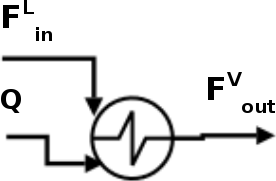
\includegraphics[scale=0.5]{images/Chap3/esquemareboilersteady2.png}
\caption{Modelo esquemático de um refervedor estacionário.}
\label{fig:reboilersteady}
\end{figure}

O modelo é composto pelas seguintes equações:

\begin{flushleft}
Balanço de massa:
\end{flushleft}
\begin{equation}
F_{in}^L = F_{out}^V
\end{equation}
\begin{equation}
x_{in_i} = y_{out_i} \qquad i=1,2,\cdots,c
\end{equation}
Balanço de energia:
\begin{equation}
F_{in}^L \cdot h_{in}^L + Q= F_{out}^V \cdot h_{out}^V 
\end{equation}
Queda de pressão:
\begin{equation}
\Delta P = P_{in}^L - P_{out}^V
\end{equation}
As propriedades físicas e termodinâmicas necessárias são calculadas através de rotinas externas:
\begin{equation}
h_{out}^L = h^L(T_{out}^L, P_{out}^L, x_{out})
\end{equation}
\begin{equation}
h_{out}^V = h^V(T_{out}^V, P_{out}^V, y_{out})
\end{equation}
\begin{equation}
v^V = v^V(T_{out}^V, P_{out}^V, y_{out})
\end{equation}
\begin{equation}
\rho^V = \rho^V(T_{out}^V, P_{out}^V, y_{out})
\end{equation}

A implementação do modelo na linguagem do simulador \emso\ é apresentada no
\autoref{code:refervedorestacionario}.
\lstinputlisting[firstline=119, lastline=149, numbers=none, language=EMSO, caption=Modelo de refervedor estacionário. ,
label=code:refervedorestacionario] {images/Chap4/reboiler.mso}

\section{Condensadores}
Colunas de destilação podem possuir vários tipos de condensadores e
refervedores.
Em alguns casos, os condensadores possuem um acúmulo significativamente
maior que o acúmulo dos pratos. Este fato contribui para uma maior estabilidade
operacional do equipamento.
Esta variedade de configurações leva a
diferentes comportamentos dinâmicos e exerce um grande efeito no comportamento da coluna \cite{Kooijman:1995a}.

Neste trabalho, dois modelos de condensadores foram construídos: um modelo
dinâmico em equilíbrio termodinâmico, representando um condensador parcial;
e um modelo estacionário com condensação total, que pode ser integrado a um modelo de tanque
de acúmulo para o comportamento dinâmico.

\subsection{Condensador Dinâmico ou Parcial} \label{sec:modelocondensadordinamico}
Na literatura, são encontrados modelos tradicionais e consolidados deste tipo de equipamento. Geralmente o condensador
dinâmico é
modelado como mais um estágio de equilíbrio. Alguns simuladores comerciais usam modelos mais rigorosos de troca térmica
que consideram o condensador dividido em duas regiões: uma região de condensação do fluido e outra região de
sub-resfriamento do mesmo. O modelo de condensador desenvolvido é relativamente simples, com
as considerações de equilíbrio termodinâmico entre as fases e que as mesmas (fase líquida e fase vapor) estão
em condição de mistura perfeita. No equipamento entra uma corrente totalmente vaporizada e duas correntes saem,
uma líquida e outra na fase vapor. Trata-se de um modelo de condensador parcial cujo desenho esquemático por ser
visto na \autoref{fig:condenser}:

\begin{figure}[htb]
\centering 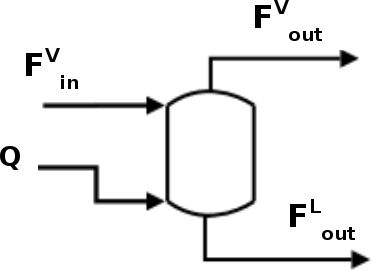
\includegraphics[scale=0.5]{images/Chap3/esquemacondenser2.png}
\caption{Modelo esquemático de um condensador parcial dinâmico.}
\label{fig:condenser}
\end{figure}

O equacionamento básico é mostrado a seguir.

Balanço molar por componente:
\begin{equation}
\dfrac{dM_i}{dt} = F_{in}^V \cdot y_{in_i} - F_{out}^L  \cdot x_{out_i} - F_{out}^V \cdot y_{out_i}  \qquad i=1,2,\cdots,c
\end{equation}
Balanço de energia:
\begin{equation}
\dfrac{dE}{dt} = F_{in}^V \cdot h_{in}^V - F_{out}^L  \cdot h_{out}^L - F_{out}^V \cdot h_{out}^V + Q
\end{equation}
Acúmulos:
\begin{equation}
M_i = M^L \cdot x_{out_i} + M^V \cdot y_{out_i}  \qquad i=1,2,\cdots,c
\end{equation}
\begin{equation}
E = M^L \cdot h_{out}^L + M^V \cdot h_{out}^V - P_{out}^L \cdot V_{cond}
\end{equation}
\nomenclature{$V_{cond}$}{Volume do condensador \nomunit{m^3}}
Restrições das frações molares:
\begin{equation}
\sum_i x_{out_i} = 1
\end{equation}
\begin{equation}
\sum_i x_{out_i} = \sum_i y_{out_i}
\end{equation}
Equilíbrio químico, mecânico e térmico:
\begin{equation}
\hat{\phi}_i^L \cdot x_{out_i} = \hat{\phi}_i^V \cdot y_{out_i}  \qquad i=1,2,\cdots,c
\end{equation}
\begin{equation}
P_{out}^L = P_{out}^V
\end{equation}
\begin{equation}
T_{out}^L = T_{out}^V
\end{equation}
\nomenclature{$T_{out}^L$}{Temperatura de saída da corrente de líquido \nomunit{K}}
\nomenclature{$T_{out}^V$}{Temperatura de saída da corrente de vapor \nomunit{K}}
Restrição geométrica:
\begin{equation}
V_{cond} = M^L \cdot v^L + M^V \cdot v^V
\end{equation}
Nível de líquido:
\begin{equation}
Level = \dfrac {M^L \cdot v^L}{A_{cross}}
\end{equation}

As propriedades físicas e termodinâmicas necessárias são calculadas através de rotinas externas:
\begin{equation}
h_{out}^L = h^L(T_{out}^L, P_{out}^L, x_{out})
\end{equation}
\begin{equation}
h_{out}^V = h^V(T_{out}^V, P_{out}^V, y_{out})
\end{equation}
\begin{equation}
v^L = v^L(T_{out}^L, P_{out}^L, x_{out})
\end{equation}
\begin{equation}
v^V = v^V(T_{out}^V, P_{out}^V, y_{out})
\end{equation}
\begin{equation}
\hat{\phi}_i^L = \hat{\phi}_i^L(T_{out}^L, P_{out}^L, x_{out})  \qquad
i=1,2,\cdots,c
\end{equation}
\begin{equation}
\hat{\phi}_i^V = \hat{\phi}_i^V(T_{out}^V, P_{out}^V, y_{out})  \qquad
i=1,2,\cdots,c
\end{equation}

No \autoref{code:condensadordinamico}, é apresentada a implementação do modelo de condensador dinâmico na linguagem de
modelagem do simulador \emso.
\lstinputlisting[firstline=43, lastline=105, numbers=none, language=EMSO, caption=Modelo de condensador dinâmico. ,
label=code:condensadordinamico] {images/Chap4/condenser.mso}

\subsection{Condensador Estacionário ou Total} \label{sec:modelocondensadorestacionario}
O desenho esquemático de um condensador estacionário pode ser visto na \autoref{fig:condsteady}. O modelo desenvolvido
considera que o equipamento recebe uma corrente totalmente vaporizada e com a retirada de calor, condensa totalmente a
mesma.
\begin{figure}[htb]
\centering 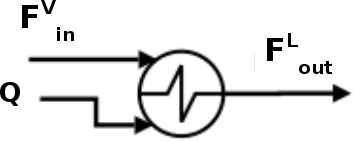
\includegraphics[scale=0.5]{images/Chap3/esquemacondensersteady2.png}
\caption{Modelo esquemático de um condensador estacionário.}
\label{fig:condsteady}
\end{figure}

O modelo é representado pelas seguintes equações:

\begin{flushleft}
Balanço de massa:
\end{flushleft}
\begin{equation}
F_{in}^V = F_{out}^L
\end{equation}
\begin{equation}
y_{in_i} = x_{out_i}  \qquad i=1,2,\cdots,c
\end{equation}
Balanço de energia:
\begin{equation}
F_{in}^V \cdot h_{in}^V + Q = F_{out}^L \cdot h_{out}^L 
\end{equation}
Queda de pressão:
\begin{equation}
\Delta P = P_{in}^V - P_{out}^L
\end{equation}
As propriedades físicas e termodinâmicas necessárias são calculadas através de rotinas externas:
\begin{equation}
h_{out} = h(T_{out}, P_{out}, z_{out})
\end{equation}

O modelo de condensador estacionário, implementado no \emso , pode ser visualizado no
\autoref{code:condensadorestacionario}.
\lstinputlisting[firstline=110, lastline=132, numbers=none, language=EMSO, caption=Modelo de condensador estacionário. ,
label=code:condensadorestacionario] {images/Chap4/condenser.mso}

\section{Prato - Estágio de Equilíbrio} \label{sec:modeloprato}
O modelo de prato representa um estágio de equilíbrio de uma coluna de destilação. Como mostrado no
\autoref{chap:revisaobibliografica}, existem diversas linhas de modelagem de um estágio de equilíbrio.
Dentro da categoria de modelos rigorosos com consideração de equilíbrio termodinâmico entre as fases, o
ponto de maior variação entre os modelos está nas equações relacionadas com a hidrodinâmica do prato,
isto é, nas correlações para o cálculo das vazões internas dos pratos, perfis de pressão e outros
detalhes hidráulicos.
A construção do modelo desenvolvido neste trabalho incluiu a consulta e análise
de inúmeras fontes da literatura, utilizando como base o
trabalho de \citeonline{Gani:1986}.
As correntes envolvidas no modelo são apresentadas no diagrama da
\autoref{fig:prato}:

\begin{figure}[htb]
\centering 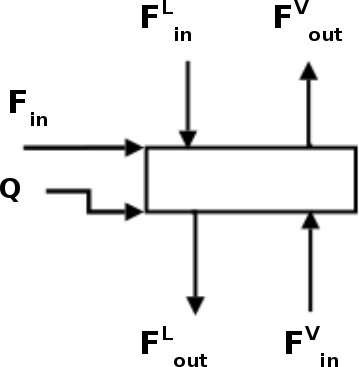
\includegraphics[scale=0.5]{images/Chap3/esquemaprato2.png}
\caption{Modelo esquemático de um prato.}
\label{fig:prato}
\end{figure}

Poderia-se adicionar ainda, uma corrente material de retirada lateral no prato. Com esta corrente ficaria mais fácil
simular colunas que possuem retiradas e refluxos intermediários, comuns na destilação de petróleo. Enquanto esta
corrente adicional não é implementada, deve utilizar um separador de correntes entre pratos de uma coluna e o mesmo
resultado será obtido.

O modelo de prato é composto pelas seguintes equações:
\begin{flushleft}
Balanço molar por componente:
\end{flushleft}
\begin{equation}
\dfrac{dM_i}{dt} = F_{in} \cdot z_{in_i} + F_{in}^L \cdot x_{in_i} + F_{in}^V \cdot y_{in_i} - F_{out}^L  \cdot x_{out_i} -
F_{out}^V \cdot y_{out_i}  \qquad i=1,2,\cdots,c
\end{equation}
Balanço de energia:
\begin{equation}
\dfrac{dE}{dt} = F_{in} \cdot h_{in} + F_{in}^L \cdot h_{in}^L + F_{in}^V \cdot h_{in}^V - F_{out}^L  \cdot h_{out}^L -
F_{out}^V \cdot h_{out}^V + Q
\end{equation}
Acúmulos:
\begin{equation}
M_i = M^L \cdot x_{out_i} + M^V \cdot y_{out_i}  \qquad i=1,2,\cdots,c
\end{equation}
\begin{equation}
E = M^L \cdot h_{out}^L + M^V \cdot h_{out}^V - P_{out}^L \cdot V_{tray}
\end{equation}
\nomenclature{$V_{tray}$}{Volume do prato \nomunit{m^3}}
Restrições das frações molares:
\begin{equation}
\sum_i x_{out_i} = 1
\end{equation}
\begin{equation}
\sum_i x_{out_i} = \sum_i y_{out_i}
\end{equation}
Equilíbrio químico, mecânico e térmico:
\begin{equation}
\hat{\phi}_i^L \cdot x_{out_i} = \hat{\phi}_i^V \cdot y_{eq_i}  \qquad
i=1,2,\cdots,c
\end{equation}
\begin{equation}
P_{out}^L = P_{out}^V
\end{equation}
\begin{equation}
T_{out}^L = T_{out}^V
\end{equation}
Eficiência de Murphree:
\begin{equation}
E_{MV_i} = \dfrac{ y_{out_i} - y_{in_i} } {y_{eq_i} - y_{in_i} } \qquad i=1,2,\cdots,c
\end{equation}
\nomenclature{$E_{MV}$}{Eficiência de prato de Murphree}
Restrição geométrica:
\begin{equation}
V_{tray} = M^L \cdot v^L + M^V \cdot v^V
\end{equation}
Nível de líquido:
\begin{equation}
Level = \dfrac {M^L \cdot v^L}{A_p}
\end{equation}
onde, $A_p$ é a área útil do prato (área do total do prato - área do
\textit{downcomer}), $V_{tray}$ é o volume total do prato, $Level$ é o nível de
líquido e $y_{eq_i}$ é a composição do vapor que está em equilíbrio com o líquido.

\nomenclature{$A_p$}{Área do prato (Área do total do prato -  Área do \textit{downcomer}) \nomunit{m^2}}

Ainda são necessárias duas equações para o cálculo das vazões de líquido e vapor do prato que são função
das propriedades físicas dos fluidos, da geometria do prato, da queda de pressão e do acúmulo de líquido
em cada estágio:
\begin{equation}
F^L = f(M, \textrm{geometria}, \textrm{propriedades fisicas})
\end{equation}
\begin{equation}
F^V = f(\Delta P, \textrm{geometria}, \textrm{propriedades fisicas})
\end{equation}
\nomenclature{$F^L$}{Vazão molar de líquido \nomunit{mol/s}}
\nomenclature{$F^V$}{Vazão molar de vapor \nomunit{mol/s}}

Na \autoref{sec:hydraulics}, é apresentada uma discussão a cerca das
diversas correlações encontradas na literatura para o cálculo da hidrodinâmica do prato.

As propriedades físicas e termodinâmicas necessárias são calculadas através de rotinas externas:
\begin{equation}
h_{out}^L = h^L(T_{out}^L, P_{out}^L, x_{out})
\end{equation}
\begin{equation}
h_{out}^V = h^V(T_{out}^V, P_{out}^V, y_{out})
\end{equation}
\begin{equation}
v^L = v^L(T_{out}^L, P_{out}^L, x_{out})
\end{equation}
\begin{equation}
v^V = v^V(T_{out}^V, P_{out}^V, y_{out})
\end{equation}
\begin{equation}
\rho^L = \rho^L(T_{out}^L, P_{out}^L, x_{out})
\end{equation}
\begin{equation}
\rho^V = \rho^V(T_{out}^V, P_{out}^V, y_{out})
\end{equation}
\begin{equation}
\hat{\phi}_i^L = \hat{\phi}_i^L(T_{out}^L, P_{out}^L, x_{out})  \qquad
i=1,2,\cdots,c
\end{equation}
\begin{equation}
\hat{\phi}_i^V = \hat{\phi}_i^V(T_{out}^V, P_{out}^V, y_{eq}) \qquad
i=1,2,\cdots,c
\end{equation}

O modelo de estágio de equilíbrio foi implementado no simulador \emso\ em etapas. Um modelo básico foi construído com as
equações correspondentes aos balanços e às relações de equilíbrio. O modelo complementar contém as equações da
hidrodinâmica. O \autoref{code:prato} apresenta os modelos.
\lstinputlisting[firstline=38, lastline=154, numbers=none, language=EMSO, caption=Modelos de prato. , label=code:prato]
{images/Chap4/tray.mso}

Com esta divisão, o desenvolvimento de novos modelos de prato fica facilitado. Esta estrutura, baseada no conceito de
herança, ilustrado no \autoref{ap:emso}, permite a reutilização do código presente no modelo básico.
Assim, qualquer modelo novo de estágio de
equilíbrio pode se basear no modelo de prato básico, como o anteriormente apresentado, através da instrução:
\vspace{0.5cm}
\lstinputlisting[firstline=108, lastline=109, numbers=none, caption=Exemplo de modelagem baseada em herança.,
language=EMSO] {images/Chap4/tray.mso}
e conter apenas as novas equações para as vazões internas da coluna.

\section{Colunas de Destilação} \label{sec:modelocolunas}
Com os modelos dos acessórios apresentados anteriormente, várias configurações de colunas podem ser montadas, de acordo
com o equipamento real a ser modelado. Pode ser modelada desde uma simples seção de coluna (Figura
\autoref{fig:secaocoluna}) até uma coluna com condensador e refervedor dinâmicos (Figura \autoref{fig:colunadinamica}).

\begin{figure}[htb]
\centering
  \subfloat[Seção de coluna]{\label{fig:secaocoluna} 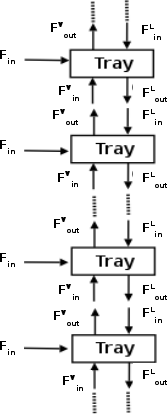
\includegraphics[scale=0.55]{images/Chap3/section2.png}}
  \qquad
  \subfloat[Coluna completa]{\label{fig:colunadinamica} 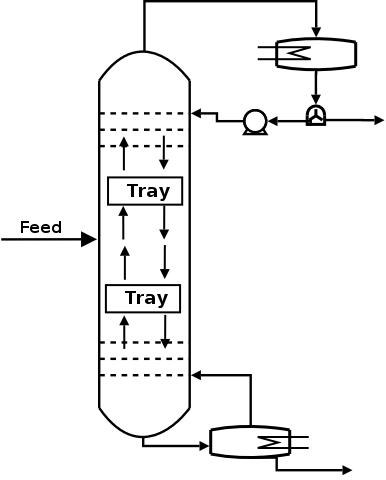
\includegraphics[scale=0.3]{images/Chap3/distKettlecond.png}}
  \caption{Diferentes configurações de colunas de destilação.}
  \label{fig:colunas}
\end{figure}

Para a construção de colunas de destilação com retiradas laterais e refluxos externos, como já mencionado
na \autoref{sec:modeloprato}, deve-se adicionar separadores de correntes entre os pratos, já que o modelo de
estágio de equilíbrio não contém um corrente de saída extra.
O \autoref{code:secao} corresponde à implementação de uma seção de coluna, como a apresentada na Figura
\autoref{fig:secaocoluna}, na linguagem de modelagem do \emso\ . O \autoref{code:colunadinamica} corresponde à
implementação de uma coluna de
destilação como a apresentada na Figura \autoref{fig:colunadinamica}, também
na linguagem do simulador.
\lstinputlisting[firstline=46, lastline=67,
numbers=none, language=EMSO, caption=Modelo de seção de coluna de destilação. , label=code:secao] {images/Chap4/column.mso}

Como pode ser visto na implementação acima, além dos parâmetros necessários para a utilização de cálculos
termodinâmicos externos ($NComp$: número de componentes e $PP$: pacote de propriedades termodinâmicas),
foram declarados alguns parâmetros adicionais: \textit{topdown}, \textit{top} e \textit{bot}.
Estes parâmetros são utilizados para auxiliar nas conexões das correntes internas das colunas. O usuário é responsável
por fornecer o valor de \textit{topdown}, que deve ser 1 se a contagem dos pratos da coluna começa pelo topo
ou -1 se a contagem dos pratos começa pelo fundo. Os parâmetros \textit{top} e \textit{bot} representam
o prato do topo e do fundo da coluna respectivamente. Assim, se $topdown = 1$ o prato do topo é o prato $1$ ($top=1$)
e o prato do fundo o $NTrays$  ($bot = NTrays$). Por outro lado, se $topdown = -1$ o prato do topo
é o prato $NTrays$ ($top=NTrays$) e o prato do fundo o $1$ ($bot = 1$). Esta convenção é necessária para
a realização das conexões entre as vazões dos estágios bem como a visualização dos resultados gerados na simulação.

A conexão entre os $NTrays$ pratos da torre é realizada na seção \textit{CONNECTIONS}. A vazão de vapor que
deixa o prato inferior é conectada à vazão de vapor que entra no prato superior assim como a vazão de líquido
que escoa do prato superior é ligada à vazão de líquido que entra no prato inferior. Com estas conexões, as vazões
internas de uma seção de coluna ficam determinadas e o modelo representado pela Figura \autoref{fig:secaocoluna} é
construído.

\lstinputlisting[firstline=77, lastline=125, numbers=none, language=EMSO, caption=Modelo de coluna de destilação com
condensador e refervedor dinâmicos. , label=code:colunadinamica] {images/Chap4/column.mso}

Vale ressaltar que os modelos de coluna acima apresentados foram construídos com base no conceito de composição
da programação orientada a objetos. Esta característica da linguagem fica evidente quando são declaradas
como variáveis do modelo da coluna outros modelos básicos já existentes, por exemplo:
\lstinputlisting[firstline=91, lastline=97, numbers=none, caption=Exemplo de modelagem baseada em composição.,
language=EMSO] {images/Chap4/column.mso}

Podem ser construídas colunas de destilação de diversas configurações, basta
declarar, na seção de variáveis, diferentes tipos de condensadores,
refervedores e tanques de acúmulo.
Por exemplo, com os modelos básicos apresentados neste capítulo pode-se montar
facilmente uma torre com condensador e refervedor estacionários e tanques no topo e fundo:
\lstinputlisting[firstline=1, lastline=10, numbers=none, caption= Outro exemplo de modelagem baseada em composição.,
language=EMSO] {images/Chap4/composicao.mso}
A diferença entre os modelos está apenas nos tipos de acessórios das colunas e nas conexões entre as correntes internas
da mesma.

No \autoref{code:colunadinamica}, as conexões necessárias, de acordo com a Figura \autoref{fig:colunadinamica}, são:
\begin{itemize}
 \item a conexão da corrente de saída de vapor do refervedor com a entrada de vapor do prato de fundo da coluna;
 \item a conexão da saída de vapor do prato inferior à entrada de vapor do prato superior, ao longo de
todos os pratos da coluna;
 \item a conexão da saída de vapor do prato de topo da columa com a entrada de vapor do condensador;
 \item a conexão da saída de líquido do condensador na entrada de um \textit{splitter};
 \item a conexão de uma das saídas do \textit{splitter} com a entrada da bomba (a outra saída do \textit{splitter} é a
corrente de destilado);
 \item a conexão da saída da bomba com a entrada de líquido do prato do topo da coluna;
 \item a conexão da saída de líquido do prato superior com a entrada de líquido do prato inferior, ao longo de toda
a coluna;
 \item a conexão da saída de líquido do prato do fundo na entrada de líquido de refervedor.
\end{itemize}


\section{Hidráulica de Pratos}\label{sec:hydraulics}
Uma coluna de destilação consiste de um cilindro vertical com diâmetro que pode variar de poucos centímetros
a alguns metros. Da mesma maneira, o número de pratos de uma torre pode variar de poucas unidades  a
várias dezenas.

Uma característica geral do escoamento na bandeja é o fato de que o líquido é impedido de escoar para
o prato abaixo através dos furos pela vazão ascendente de vapor. Assim, enquanto o vapor flui verticalmente
entre os pratos, o líquido escoa horizontalmente na superfície da bandeja caracterizando o fluxo cruzado.
Os três principais tipos de pratos encontrados em unidades industriais são:
pratos perfurados, valvulados, e pratos com borbulhadores. Na
\autoref{fig:traytypes} são mostradas as diferentes aberturas encontradas nesses pratos e o caminho a ser realizado pelo vapor para atravessá-lo.
\begin{figure}[htb]
\centering 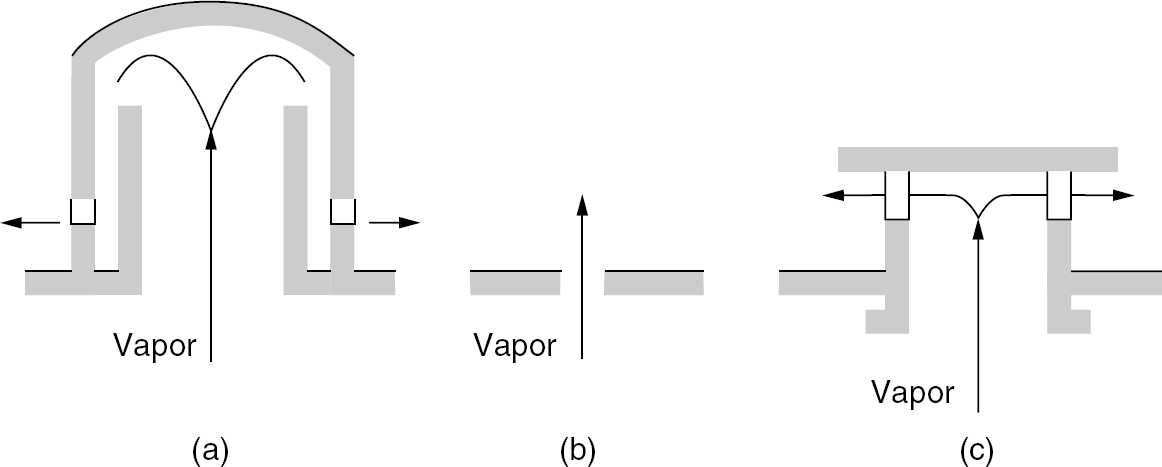
\includegraphics[scale=0.5]{images/Chap3/traytype.png}
\caption{Diferentes tipos de aberturas dos pratos: (a) borbulhadores, (b)
furo e (c) válvula.}
\label{fig:traytypes}
\end{figure}

Apesar das diferentes configurações de colunas de destilação de pratos, todas possuem
características em comum que permitem que as mesmas sejam descritas de uma maneira generalizada através
de uma modelagem mais simplificada. Estas generalizações são importantes para o estudo do comportamento
hidráulico do prato mesmo em se tratando de um tipo específico de bandeja. Isto deve-se ao fato da alta
complexidade de análise do fluxo cruzado que acontece entre o líquido e o vapor. Sendo assim,
sempre são feitas algumas considerações simplicativas na elaboração de correlações de queda de pressão
e vazão de líquido \cite{Khoury:2005}.

Os principais fatores que influenciam o desempenho do prato são: a formação de espuma, o arraste de líquido e vapor,
o gradiente na concentração de líquido no prato, gotejamento, inundação e a queda de pressão.
Quando é realizado o projeto de uma coluna de destilação todos estes fatores são considerados pois a maioria
deles é conseqüência da capacidade da coluna e das vazões internas de líquido e vapor que caracterizam o ponto
de operação a que a mesma será submetida.
Diversos níveis de modelagem podem ser realizados considerando todos ou parte destes fatores citados.
Modelos rigorosos com simplificações na hidráulica levam em conta
apenas a formação de bolhas, que afeta diretamente a quantidade de líquido no prato e conseqüentemente
o seu grau de aeração, e a queda de pressão do equipamento.

Nas próximas seções serão apresentadas as principais correlações de hidrodinâmica encontradas na literatura e uma
discussão sobre as mesmas.

\subsection{Vazão de vapor - Queda de Pressão}\label{sec:vapflow}
A força motriz para o escoamento do líquido em uma torre é a força da gravidade. Já para o escoamento de vapor acontecer
deve existir uma diferença de pressão ao longo da coluna. Assim, os pratos inferiores devem ser mantidos em uma
pressão superior aos do topo. Além disso, um gradiente mínimo de pressão é
necessário para evitar gotejamento de líquido através das aberturas dos pratos \cite{Khoury:2005}.

Segundo \citeonline{Lockett:1986} a queda de pressão em um estágio, $h_{WT}$, é a soma de três contribuições,
aqui representadas em termos da altura de líquido (\textit{head}):
\begin{equation}
h_{WT} = h_{DT}+h_{cl}+h_R
\end{equation}
onde $h_{DT}$ representa a queda de pressão do prato seco, isto é, a resistência ao escoamento do vapor mesmo quando
não há líquido no prato; $h_{cl}$ é a queda de pressão devido ao acúmulo de líquido claro e $h_R$ é uma queda de pressão
residual referente à tensão superficial dos fluidos.

Ainda segundo \citeauthoronline{Lockett:1986}, a queda de pressão do prato seco pode ser calculada por:
\begin{equation}
h_{DT} = \dfrac{\xi \rho_{vap} u^2_ h}{2 g \rho_{liq}}
\end{equation}
onde $u_ h$ é a velocidade do vapor através dos furos do prato e $\xi$ é o chamado coeficiente de orifício,
que é uma função principalmente do número de Reynolds do orifício $Re_h$
e de parâmetros geométricos do prato. Para uma visão mais detalhada sobre correlações para o cálculo de $\xi$ e $h_{DT}$,
ver \citeonline{Lockett:1986}.
\nomenclature{$g$}{Aceleração da gravidade\nomunit{m/s^2}}
A contribuição da altura de líquido para a queda de pressão pode ser calculada por:
\begin{equation}
h_{cl} = \dfrac{\left( P_1 - P_2\right) + u_S \rho^V \left(u_h - u_S \right) }{g \rho^L}
\end{equation}
onde $P_1$ é a pressão no fundo do prato, $P_2$ é a pressão acima do líquido,
$u_ S$ é a velocidade superficial do vapor e $g$ é a aceleração da gravidade.

Existem diversas correlações para a queda de pressão residual. Os fatores mais relevantes na sua determinação
são as propriedades físicas dos fluidos e a razão espessura do prato/diâmetro do furo. Devido à sua pequena
contribuição, para pratos valvulados este termo pode ser ignorado sem maiores problemas. Já para pratos perfurados
pode ser calculada de uma forma simplificada por:
\begin{equation}
h_{R} = \dfrac{4\sigma }{d_h \rho^L g}
\end{equation}
onde $\sigma$ corresponde à tensão superficial do líquido e $d_h$ ao diâmetro do furo.

Apesar de todo o rigorismo proposto para o cálculo da queda de pressão do prato, geralmente são utilizadas correlações
mais simplificadas na construção de modelos. A contribuição da tensão superficial é geralmente ignorada e
a queda de pressão
do prato seco se resume a um parâmetro. A pressão devido ao acúmulo de líquido é calculada através da fórmula
convencional de pressão hidrostática. Sendo assim, o $\Delta P$ se resume a uma equação que é função da altura
de líquido no prato, da vazão de vapor e de propriedades físicas do fluido. Na \autoref{tab:flowvapcorrelations},
as principais correlações encontradas na literatura são mostradas.
\begin{table}[p]
\caption{Correlações para cálculo da queda de pressão em função da vazão de vapor.}
\label{tab:flowvapcorrelations}
\begin{center}
\begin{tabular}{lp{0.7\textwidth}} % {lp{0.5\textwidth}cc}
\hline
\textbf{Fonte} &  \hspace{0.2\textwidth}\textbf{Correlação} \\ \hline
\citeonline{Feehery:1998} &
\begin{equation}
\label{eq:feehery}
\begin{array}{l}
\Delta P = \Delta P^{static} + \Delta P^{dry} \\
\Delta P^{static} = \dfrac{V_{liq}}{A_p} \cdot \rho_{vap} \cdot g\\
\Delta P^{dry} = \rho^V \left( \dfrac{F^V \cdot Mw}{\rho^V} \cdot A_{a} \cdot w\right) ^2\\
\end{array}
\end{equation}
 \\
\hline
\citeonline{Roffel:2000} &
\begin{equation}
\begin{array}{l}
\Delta P = \Delta P^{dry} + \beta \dfrac{M \cdot Mw}{A_{cross}} \cdot g \cdot 10^5 \\
\Delta P^{dry} = 0,0013 \left( \dfrac{F^V \cdot Mw}{\rho^V \cdot A_{h}}\right) ^{1,08}\\
% \cdot bar \left(\dfrac{s}{m}\right)^{1.08} \cdot
\Delta P=bar, F^V=kmol/s, Mw=kg/kmol \\ \rho^V=kg/m^3,  A_{h}=m^2
\end{array}
\end{equation}
 \\
\hline
\citeonline{Klingberg:2000} &
\begin{equation}
\begin{array}{l}
\Delta P = \Delta P_{tr} +g \cdot \rho^L \cdot Level \\
\Delta P_{tr} = f(F_{S})\\
F_{S} = u_S \cdot \rho^{V\ 0,5} \\
u_S \cdot \rho^V \cdot A_{cross} = Mw_V \cdot F^V
\end{array}
\end{equation}
 \\
\hline
\citeonline{Reepmeyer:2003} &
\begin{equation}
\begin{array}{l}
\Delta P = \left( \dfrac{F^V \cdot v^V}{A_h}\right)^2 \cdot \dfrac{\rho^V \cdot c_w}{2} \\
\end{array}
\end{equation}
 \\
\hline
\citeonline{Wang:2003} &
\begin{equation}
\begin{array}{l}
\Delta P = \left(  \dfrac{F^V \cdot v^V}{A}\right)^2 \cdot \rho^V \cdot \alpha +  \rho^L \cdot g \cdot Level\\
\end{array}
\end{equation}
 \\
\hline
\citeonline{Elgue:2004} &
\begin{equation}
\begin{array}{l}
\Delta P = m\Delta P\\
m\Delta P = cte\ ou\\
m\Delta P = \beta^{tray} \cdot F^{V\ 2}\\
\end{array}
\end{equation}
 \\
\hline
\citeonline{Ltd.:2004} &
\begin{equation}
\begin{array}{l}
\Delta P = \left(  \dfrac{F^V}{A_h}\right)^2 \cdot \dfrac{\alpha}{\rho^V} + \beta \cdot \rho^L \cdot g \cdot Level\\
\end{array}
\end{equation}
 \\
\hline
\end{tabular}
\end{center}
\end{table}
\nomenclature{$w$}{Constante dependente da geometria do prato presente na \autoref{eq:feehery}}
Um fator importante na escolha de uma correlação para este tipo de cálculo é a análise da consistência de unidades
de medida. Na equação de \citeonline{Roffel:2000}, por exemplo, não se consegue chegar à unidade de pressão em
$\Delta P^{dry}$ sem que seja atribuída uma unidade à constante $0,0013$.

Outra consideração importante na análise das correlações é o seu grau de rigorismo. Se comparadas ao método
de cálculo de \citeonline{Lockett:1986}, as equações apresentadas são todas
simplificadas. Mesmo assim, pode-se dividir estas equações em dois subconjuntos:
as que consideram apenas a contribuição da vazão de vapor e da queda de pressão do prato seco e as que consideram adicionalmente a queda de pressão estática da coluna
de líquido do prato.

Neste trabalho as correlações de \citeonline{Reepmeyer:2003} e \citeonline{Wang:2003} foram implementadas e
comparadas. Para a comparação foram utilizados dados reais de operação de uma coluna deisobutanizadora,
comparando-se os perfis de temperatura e pressão ao longo da coluna.
A equação de \citeonline{Reepmeyer:2003} apresentou melhores resultados mas não mostrou muita
robustez em algumas simulações. Pois, pequenas variações no parâmetro $c_w$, envolvido nesta correlação,
são capazes de gerar grandes impactos na resposta do modelo. Além disso, esta correlação
apresentou uma maior freqüência de falhas numéricas nos testes realizados.
Por outro lado, a equação de \citeonline{Wang:2003} se apresentou mais estável por contar com a contribuição da pressão estática à pressão total. O termo ($\rho^L \cdot g \cdot Level$)
confere à correlação um amortecimento às variações da vazão de vapor, que são muito grandes
quando se trata de um procedimento de partida de uma coluna.
Porém, como a primeira correlação apresentou melhores resultados na comparação entre dados experimentais \textit{versus}
modelo, esta foi a escolhida neste estudo.

Outra consideração importante é que a equação explícita em $\Delta P$
deixa o sistema de equações mais propenso a falhas de integração do que a correlação explícita em $F$.
Finalmente, após a análise das equações apresentadas, a forma final da equação que é utilizada neste estudo é:
\begin{equation}
\label{eq:vapfinal}
F^V = \dfrac{A_h}{v^V} \cdot \sqrt{\dfrac{\left( P_{in}^V - P_{out}^V\right)}{\rho^V \cdot \alpha}}
\end{equation}
onde, $A_h$ é a área total dos furos do prato e $\alpha$ é o coeficiente de
queda de pressão no prato seco, utilizado como parâmetro de ajuste.

\nomenclature{$h_{cl}$}{Altura de líquido claro no prato \nomunit{m}}
\nomenclature{$u_h$}{Velocidade do vapor através dos furos do prato \nomunit{m/s}}
\nomenclature{$u_S$}{Velocidade superficial do vapor: ($\frac{Q_h}{A_a}$) \nomunit{m/s}}
\nomenclature{$Q_h$}{Vazão volumétrica de vapor através dos furos do prato \nomunit{m^3/s}}
\nomenclature[G]{$\xi$}{Coeficiente de orifício}
\nomenclature{$c_w$}{Resistência ao escoamento de vapor}
\nomenclature[G]{$\sigma$}{Tensão superficial \nomunit{N/m}}
\nomenclature{$d_h$}{Diâmetro do furo \nomunit{m}}
\nomenclature[G]{$\beta^{tray}$}{Constante relacionada com propriedades físicas do prato}
\nomenclature[G]{$m\Delta P$}{Modelo para o cálculo da queda de pressão \nomunit{Pa}}
\nomenclature{$F_S$}{Fator superficial \nomunit{kg^{0.5}/m^{0.5}/s}}
\nomenclature{$A_h$}{Área total dos furos do prato \nomunit{m^2}}
\nomenclature{$P_{out}^V$}{Pressão da corrente de vapor que sai do equipamento \nomunit{atm}}
\nomenclature{$P_{out}^L$}{Pressão da corrente de líquido que sai do equipamento \nomunit{atm}}
\nomenclature{$P_{in}^V$}{Pressão da corrente de vapor que entra no equipamento \nomunit{atm}}
\nomenclature{$P_{in}^L$}{Pressão da corrente de líquido que entra no equipamento \nomunit{atm}}
\nomenclature[G]{$\alpha$}{Coeficiente de queda de pressão no prato seco}
\nomenclature[G]{$\Delta P$}{Diferença de pressão \nomunit{atm}}

\subsection{Vazão de líquido}\label{sec:liqflow}
A predição do acúmulo de líquido em cada prato e também do seu escoamento através do vertedouro é muito importante
na previsão do comportamento hidráulico de uma coluna de destilação. A altura de líquido exerce influência na
queda de pressão, eficiência do prato, nos limites de operação da coluna e no regime de escoamento do estágio.
O cálculo
da altura de líquido depende das propriedades da mistura e de parâmetros
geométricos tais como a altura e comprimento do vertedouro, a área de furos do prato, o diâmetro dos furos e outros.
As correlações existentes para a predição da altura de líquido são todas empíricas e, segundo \citeonline{Wijn:1999},
não são consideradas satisfatórias.

Existem vários trabalhos na literatura descrevendo a relação entre a altura de líquido, a quantidade
de vapor disperso na fase líquida e a sua vazão. Os métodos mais antigos expressam a altura de líquido como uma
função linear da altura do vertedouro e dos acúmulos de líquido e vapor. Nesta linha, outros
trabalhos evoluíram
da relação linear para uma função exponencial envolvendo também alguns parâmetros geométricos do prato. Depois, a altura
de líquido passou a ser considerada como a contribuição de duas parcelas, uma abaixo e outra acima do vertedouro
\cite{Wijn:1999}.

Dependendo do regime de operação da coluna (regime de \textit{spray} ou regime de bolhas, por exemplo),
o transporte
do líquido para o prato inferior pode acontecer de várias maneiras além do simples escoamento do líquido através
do vertedouro. Assim, a complexidade na modelagem desse transporte pode variar de uma relação clássica baseada na
equação de Francis (\autoref{eq:francis}) até a previsão de respingos de líquido
ocasionados pelo rompimento de bolhas em um regime de \textit{spray}.
% \begin{equation}
% F_{outL} \cdot Mw = \rho_{liq}  \cdot lw \cdot \left( \dfrac{h_{ow}}{750}\right)^{1,08}
% \end{equation}
% com $F_{outL}$ em $kmol/h$, $Mw$ em $kg/kmol$, $\rho_{liq}$ em $kg/m^3$, $lw$ em $m$ e $h_{ow}$ em $mm$.

No trabalho de \citeonline{Klingberg:2000}, a altura de líquido, $Level$, é calculada pela contribuição da
altura do vertedouro, $h_w$, e da altura da dispersão de líquido e vapor acima do mesmo, $h_{ow}$, sendo relacionada
com a vazão através da expressão:
\begin{equation}
h_{ow} = \dfrac{1,45}{g^{\frac{1}{3}}} \left( \dfrac{\frac{F_{out}^L}{lw}}{\varepsilon_l}\right)^{\frac{2}{3}} + \dfrac{c}{2g\left( \rho^V - \rho^L \right)} \left( \dfrac{F_S - 0,2\sqrt{\rho^V}} {1 - \varepsilon_l} \right)^2 
\end{equation}
onde $\varepsilon_l$ é a fração de líquido na espuma e $c$ é uma constante adimensional.
\nomenclature[G]{$\varepsilon_l$}{Fração de líquido na espuma}
\nomenclature[G]{$\varepsilon_w$}{Fração de vapor na espuma que escoa sobre o vertedouro}

Em \citeonline{Lockett:1986}, a mesma relação é utilizada, $Level = h_w + h_{ow}$. O nível total é uma função linear
do fator superficial, $F_S$, dos parâmetros geométricos ($h_w$, $lw$) e da
vazão volumétrica de líquido, $Q^L$:
\begin{equation}
Level = A h_w + B F_S + C \dfrac{Q^L}{lw} + D
\end{equation}
com os parâmetros $A,\ B,\ C,\ e\ D$ variando conforme o tipo de prato e mistura a ser destilada. Vários conjuntos
de valores podem ser encontrados em \citeonline{Lockett:1986}.
A altura de espuma acima do vertedouro é dada pela equação de Francis:
\begin{equation}
\label{eq:francis}
h_{ow} = \dfrac{1,04}{C_d^{0,67} g^{0,33}} \left(
\dfrac{Q^L}{\left(1-\varepsilon_w \right) lw } \right)^{0,67}
\end{equation}
onde $C_d$ é o coeficiente de descarga, $g$ é a aceleração da gravidade em
$m/s^2$, $Q^L$ é a vazão volumétrica de líquido em $m^3/s$, $lw$ o comprimento do vertedouro em $m$ e $\varepsilon_w$ é a fração de vapor na espuma que escoa sobre o
vertedouro.

Além das duas formulações mostradas anteriormente, muitas outras equações são apresentadas na literatura para o
cálculo da vazão de líquido em uma coluna de destilação. A grande maioria delas é baseada na clássica equação de
Francis, que trata de uma relação simples entre a altura de líquido e a vazão. As principais correlações
encontradas estão listadas na \autoref{tab:liqflowcorrelations}.

\begin{table}[p]
\caption{Correlações para cálculo da vazão de líquido em colunas de destilação.}
\label{tab:liqflowcorrelations}
\begin{center}
\begin{tabular}{lp{0.7\textwidth}} % {lp{0.5\textwidth}cc}
\hline
\textbf{Fonte} &  \hspace{0.2\textwidth}\textbf{Correlação} \\ \hline
\citeonline{Olsen:1997} &
\begin{equation}
\begin{array}{l}
F^L = \dfrac{lw N_p \rho^L}{Mw \left( 0,665 F_W\right)^{\frac{3}{2}} } \left( \dfrac{M^L Mw}{\rho^L A_a} - h_w \right)^{\frac{3}{2}} - P_l
\end{array}
\end{equation}
 \\
\hline
\citeonline{Feehery:1998} &
\begin{equation}
\begin{array}{l}
% F_{outL} = \dfrac{lw \rho_{liq}}{Mw} \left( \dfrac{\frac{V_{liq}}{A_p} - h_w} {750}\right)^{\frac{3}{2}}
F^L = \dfrac{lw \rho^L}{Mw} \left( \dfrac{h_{ow}} {750}\right)^{\frac{3}{2}}
\end{array}
\end{equation}
 \\
\hline
\citeonline{Roffel:2000} &
\begin{equation}
\label{eq:roffel}
\begin{array}{l}
F^L = \dfrac{2}{3} \sqrt{2g} \dfrac{\rho^L}{Mw} lw\ \phi\ h_{ow}^{\frac{3}{2}}\\
\phi = 2\beta-1 \\
\beta = 1- 0,3593 \left(\dfrac{F^V Mw} {A_{cross} \sqrt{\rho^V}} \right)^{0,177709} \\
h_{ow} = \dfrac{M^L Mw}{A_{cross} \rho^L \phi}
\end{array}
\end{equation}
 \\
\hline
\citeonline{Wang:2003} &
\begin{equation}
\label{eq:wang}
\begin{array}{l}
F^L = \alpha_w \ lw \dfrac{\left(\frac{Level - \beta h_w}{\beta} \right)^{\frac{3}{2}} }{v^L}\\
\end{array}
\end{equation}
 \\
\hline
\citeonline{Reepmeyer:2003} &
\begin{equation}
\begin{array}{l}
F^L = 1,84 \dfrac{lw}{\rho^L} \left( \dfrac{Level - h_w}{cf_w}\right)^{\frac{3}{2}} \\
\end{array}
\end{equation}
 \\
\hline
\citeonline{Ltd.:2004} &
\begin{equation}
\begin{array}{l}
F^L = 1,84 \ \rho^L \ lw \left( Level - h_w\right)^{\frac{3}{2}}
\end{array}
\end{equation}
 \\
\hline
\citeonline{Osorio:2004} &
\begin{equation}
\label{eq:osorio}
\begin{array}{l}
F^L = k_w \ d_w \ lw \left( Level - h_w\right)^{\frac{3}{2}}
\end{array}
\end{equation}
 \\
\hline
\end{tabular}
\end{center}
\end{table}
\nomenclature[G]{$\phi$}{Densidade relativa da espuma, \autoref{eq:roffel}}
\nomenclature[G]{$\alpha_w$}{Coeficiente da equação \autoref{eq:wang}, \nomunit{m^{0,5}/s}}
\nomenclature{$k_w$}{Coeficiente da \autoref{eq:osorio}, \nomunit{mol/(s\ cm^{\frac{5}{2}})}}
Na correlação de \citeonline{Olsen:1997}, $F^L$ é em $kmol/s$, $lw$ em $m$, $\rho^L$ em $kg/m^3$, $Mw$ em $kg/kmol$,
$M^L$ em $kmol$, $A_a$ em $m^2$, $h_w$ em $m$ e $P_l$ em $koml/s$. Na correlação de \citeonline{Feehery:1998}, as
unidades são: $F^L$ em $kmol/h$, $Mw$ em $kg/kmol$, $\rho^L$ em $kg/m^3$, $lw$ em $m$ e $h_{ow}$ em $mm$.
Na equação apresentada por \citeonline{Roffel:2000}, $F^L$ e $F^V$ são em $kmol/s$, $g$ é a aceleração da
gravidade em $m/s^2$, $\rho^L$ e $\rho^V$ são em $kg/m^3$, $Mw$ em $kg/kmol$, $lw$ e $h_{ow}$ em $m$,
$A_{cross}$ em $m^2$ e $M^L$ em $kmol$. Na equação de \citeonline{Wang:2003} e \citeonline{Reepmeyer:2003},
$F^L$ é expresso em $mol/s$, $lw$, $Level$ e $h_w$ em $m$, $v^L$ em $m^3/mol$ e $\rho^L$ em $kg/m^3$.
Na correlação apresentada em \citeonline{Ltd.:2004}, a equação está em base mássica com $F^L$ em $kg/s$,
$\rho^L$ em $kg/m^3$ e $lw$, $Level$ e $h_w$ em $m$. Por fim, na equação de \citeonline{Osorio:2004}, as
unidades são: $F^L$ em $mol/s$, $k_w$ em $mol/s\ cm^{\frac{5}{2}}$ e $d_w$, $lw$, $Level$ e $h_w$
em $cm$.

O grande problema das equações para o cálculo da vazão de líquido está na determinação de seus parâmetros. Quando um
modelo é construído para representar uma unidade já existente, estes parâmetros
são utilizados como parâmetros de ajuste da resposta
simulada aos dados reais de operação. Mas, quando se quer utilizar o modelo
para o projeto de um processo novo, a falta destas informações acaba inviabilizando o seu uso.
Como pode ser visto na \autoref{tab:liqflowcorrelations},
a equação de \citeonline{Roffel:2000} é a única que relaciona todas as variáveis importantes no comportamento
do líquido no prato para o cálculo da sua vazão sem envolver parâmetros
empíricos adicionais.
Porém,
% esta correlação deve ser utilizada com muito
% cuidado uma vez que envolve constantes que não são adimensionais, como o
% número $0,3593$. Neste caso,
% a utlização fica limitada às unidades de medida
% utilizadas no desenvolvimento da correlação. Além disso,
a utilização em
equipamentos com uma geometria diferente do equipamento original (utilizado na
determinação das constantes da correlação) fica comprometida.
% A equação utilizada neste trabalho foi baseada na estrutura da correlação apresentada por
% \citeonline{Wang:2003} e nos parâmetros
% da equação de \citeonline{Reepmeyer:2003}. A forma final da correlação utilizada é:
% \begin{equation}
% F_{outL} = 1,84 \ lw \dfrac{\left(\frac{Level - \beta h_w}{\beta} \right)^{\frac{3}{2}} }{v_{liq}}\\
% \end{equation}

Pelos motivos acima citados e pelo desempenho nas simulações do processo
apresentado no \autoref{chap:coldeiso}, a equação utilizada neste trabalho foi
a apresentada por \citeonline{Wang:2003}:
\begin{equation}
F^L = \alpha_w \ lw \dfrac{\left(\frac{Level - \beta h_w}{\beta} \right)^{\frac{3}{2}} }{v^L}\\
\end{equation}
onde, $\alpha_w$ e $\beta$ são parâmetros de ajuste do modelo.

\nomenclature{$cf_w$}{Resistência ao escoamento de líquido}
\nomenclature{$d_w$}{Diâmetro do vertedouro \nomunit{cm}}
\nomenclature{$V_{liq}$}{Volume de líquido no prato \nomunit{m^3}}
\nomenclature{$A_a$}{Área ativa do prato \nomunit{m^2}}
\nomenclature{$P_l$}{Vazão de produto \nomunit{kmol/s}}
\nomenclature{$Mw$}{Massa molar média da mistura\nomunit{g/mol}}
\nomenclature{$F_W$}{Correção da altura do vertedouro}
\nomenclature{$N_p$}{Número de passes}
\nomenclature{$lw$}{Comprimento do vertedouro \nomunit{m}}
\nomenclature[G]{$\beta$}{Coeficiente de aeração}
\nomenclature{$h_w$}{Altura do vertedouro \nomunit{m}}
\nomenclature{$h_{ow}$}{Altura de líquido acima do vertedouro \nomunit{m}}
\nomenclature{$Q^L$}{Vazão de líquido \nomunit{m^3/s}}
\nomenclature[G]{$\varepsilon$}{Fração de vapor na espuma}
\nomenclature{$C_d$}{Coeficiente de descarga}
% \nomenclature{$\Upsilon$}{Constante da equação de \citeonline{Wang:2003} ($m^{0,5} / s$)}
